\documentclass{article}
\usepackage{amsmath}
\usepackage{graphicx}
\title{Methodology}

\author
{
    Dereck Piché \and
    Guillermo Martinez \and
    Jonas Gabirot \and
}

\begin{document}
\maketitle

\section{Task}
Let us briefly resume our task once again in order to make this document
self-contained. Our task is to create models capable of reproducing 
the classical algorithms used by the NUPACK foundation to predict the 
free energy ($\in R$) of a DNA strand (a sequence of the elements of $\{A,C,G,T\}$).
TODO mention the size of our generated dataset

\section{Planned Methodology}
\subsection{Training dataset}
First, we will have to generate our training data. We shall implement a 
simple python script which uses the NUPACK python library in order
to generate a .json file containing our training data. We  
generated a dataset of a milion random DNA strands of length $30$, paired with their free energy as calculated by NUPACK.
\subsection{Baseline Algorithms}

\subsubsection{Multilayered Perceptron}
A multilayer perceptron (MLP) is a type of artificial neural network that consists of multiple layers of interconnected nodes organized into an input layer, one or more hidden layers, and an output layer. Each node in the MLP receives input signals from nodes in the previous layer, applies a non-linear activation function, in our case ReLU, to the weighted sum of those inputs, and passes the resulting output signal to nodes in the next layer. The weights between the nodes are learned through a process called backpropagation, where the network adjusts its internal parameters to minimize the difference between its predicted outputs and the actual target outputs. MLPs are widely used for supervised learning tasks such as classification and regression, and have been applied in areas such as computer vision, speech recognition, and natural language processing. Unlike transformers and RNNs, MLPs make no assumption about the sequential nature of the input data. In this way, an MLP is a more general algorithm and is thus well-suited to be a baseline comparison to test our assumptions about the data. For preliminary testing, we shall use an MLP with 10 hidden layers and an input size of 120, (30 bases of DNA one-hot encoded). We shall use the Adam optimizer as it is the most commonly used optimizer.

\paragraph{Cost Function}
Since this is a regression task, we shall use the Mean Squared Error (MSE) as the loss function.

\paragraph{Encoding}
To feed a string input to an MLP, we shall convert each base (A,C,T,G) to a one-hot encoded vector. With 4 categories and sequences of length 30, this gives an input size of 120.


\subsubsection{Decision trees with AdaBoost}
We might want to use this as a baseline. 


\subsection{Advanced Algorithms}

\subsubsection{Recurrent Neural Network}
Recurrent neural network (RNN) is a deep lRecurrent neural network 
(RNN) is a deep learning architecture used for sequential data prediction
using both current and past inputs. earning architecture used for sequential 
data prediction using both current and past inputs. 

it in a simple way, RRN architectures are composed of an encoder and a decoder. The initial input is vectorized by the encoder and processed as a function of the initial state, which is random at first. As a result, the encoder's weights and biases are adjusted in the form a second state to incorporate both current and past input information. The encoder recursively processes the following vectorized inputs as functions of current states, while updating the weights and biases of current states to produce new states at each iteration. The encoder terminates this recursion when it has iterated over an entire sequence of features and concludes by transmitting its final state, which incorporates all previous states, to the decoder. In the case of a many-to-one RNN underlying architecture, this paper's architecture of interest, the decoder produces one output prediction as a function of the final state received from the encoder and as a function of its own current state, random at first. By contrasting the predicted output value to the actual value of the sequence, the decoder performs gradient descent to minimize the loss function, updates its current state and backpropagates it to the encoder's states. Once the weights and biases of the encoder states are adjusted, it iterates over the following sequence of features following the same recursion procedure. This recursive process is repeated for the entire length of sequences within the training set, and the regression model is cross-validated on its ability to minimize the squared mean error between target and predicted output values in the validation and test set. 
\begin{figure}
    \caption{Illustration of RNN architecures}
    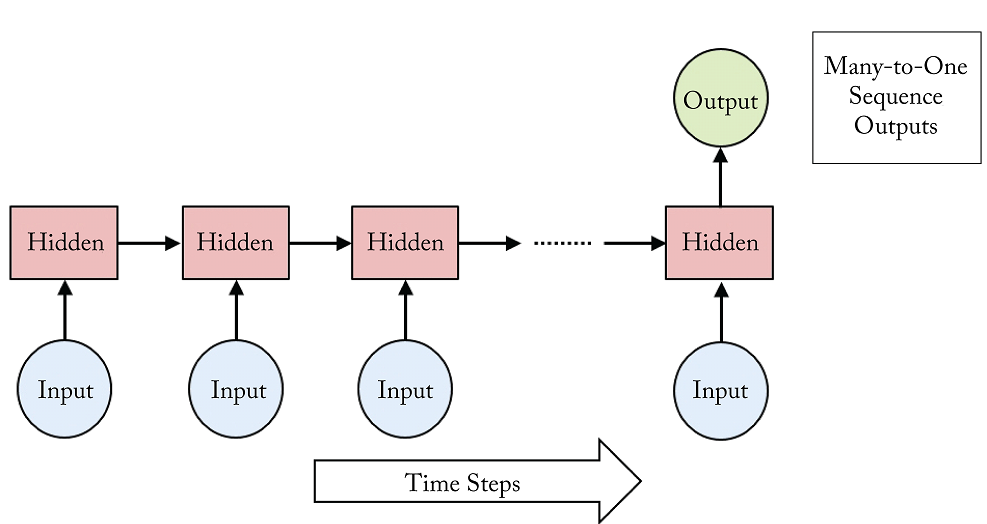
\includegraphics[width=0.7\textwidth]{images/2023-03-17-16-42-13.png}
\end{figure}

RNNs are not without challenges. In order to update parameters, the backpropagation algorithm needs to calculate gradients at each different step. This usually results in unstable neural networks due to vanishing and exploding gradients which are unable to learn long-term dependencies. Long Short Term Memory networks (LSTMs) have been proposed to avoid these problems and designed to handle long-term dependencies. Initially proposed by Hochreiter and Schmidhuber (1997),  LSTMs use cells with input, output and forget-gate to control the flow of information. 
\begin{figure}
    \caption{Long Short Term Memory cell}
    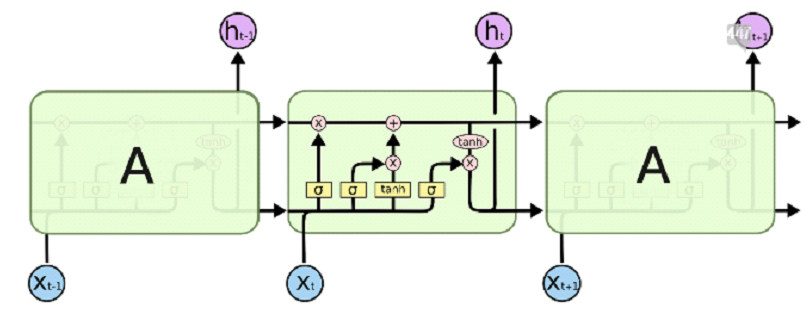
\includegraphics[width=0.7\textwidth]{images/2023-03-17-16-38-22.png}
\end{figure}



Given this paper's task to predict the level of free energy given a sequence of 30 features, we will train a many-to-one LSTMs for a regression task with multiple input time series. We will divide our entire dataset in training $80\%$, $10\%$ for testing and $10\%$ for validation. For each training instance, we will give the model a sequence of observations and a corresponding target value. The goal will be to forecast time series' free energy within the validation set. Time given, hyperparameter tuning will be performed on the validation set to optimize the choice of the learning rate, the number of units or layers, and the weight regularization techniques used as penalties on the loss function. Finally, the tunned model's prediction accuracy will be calculated on the test set using Root Mean Squared Error (RMSE) and Mean Absolute Error (MAE) metrics. 
\begin{figure}
    \caption{Information flow}
    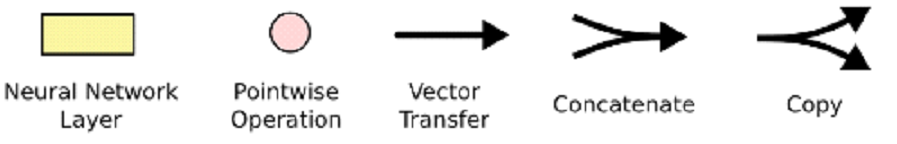
\includegraphics[width=0.7\textwidth]{images/2023-03-17-16-41-25.png}
\end{figure}

\subsubsection{Tranformer}
\paragraph{Architecture}
The transformer architecture was initially made to translate text.
However, it's subsequent use was mostly tied to token generation. 
This use only required the decoder to be part of the architecture, 
and recursively fed the predicted token in the current input while 
truncating if the input size was over the limit.
Our task is vastly different. We are dealing with a regressive task,
since we are trying to learn a function of the form $R^n \mapsto R$.
Thus, we shall only keep the decoder part of the transformer architecture. 
We only need to set the feedworward neural network in the decoder such that 
it only has one output neuron.
\paragraph{Cost Function}
Since this is a regressive task, we shall use various instances of the 
$l_p$-norm as our cost function.

\paragraph{Tokenisation, encoding, positionnal encoding}
Since the tranformer learns the embedding in the attention heads, \cite{transformers} we
shall simply use an integer mapping for the set of tokens $\{A,C,G,T\}$ as opposed to 
one-hot encoding. This is done partly due to the way the Pytorch library works.

We will train and compare our the accuracy of our decoder-only tranformer with 
respect to the absence and inclusion of positionnal embedding to the input tokens.

TODO add information on the decoder
TODO specify the training validation split

\paragraph{Advantages}
What makes the decoder-only transformer different from other models? What are
we taking advantage of by it's use? As opposed to recurrent neural networks, 
this model is less sequential in nature. We are predicting by 
taking the sequence of tokens all at once. We have high hopes for the 
distributivity of attention made possible by the head multiplicity.
We can imagine that there is high importance between the ends of the DNA 
sequence, and at the center. A transformer, given enough data, would 
be able to take advantage of this structure in order to simplify the task.


\subsection{Comparisons and analysis}
It would be more logical to compare learned models with a similar 
number of parameters. This would give us more information as 
to if the comparative advantages were caused by the particularities 
of the architecture or simply because of the increase of expressivity 
tied to bigger models.

\section{Preliminary Results and Challenges Ahead}

\subsection{Multilayered Perceptron}
Our MLP with 10 hidden layers and 88 281 parameters trained on 90\% of the data set and tested on 10\% of it gives the following results:

Epoch 1: Test MSE loss of 1.02

Epoch 2: Test MSE loss of 1.00
\section{Changes from the initial plan}
We have not strayed afar from the original plan. We 
are only more sure that time will lack to implement 
generative models like we intended after the attempt at reproducing
the aforementionned NUPACK classical algorithm.

\bibliography{bibliography}
\bibliographystyle{plain}
\end{document}
